%% Los cap'itulos inician con \chapter{T'itulo}, estos aparecen numerados y
%% se incluyen en el 'indice general.
%%
%% Recuerda que aqu'i ya puedes escribir acentos como: 'a, 'e, 'i, etc.
%% La letra n con tilde es: 'n.

\chapter{Introducci'on}

MBN es una empresa dedicada a proporcionar consultoría de negocios y desarrollo de software enfocada en apoyar a las organizaciones que requieren la adopción de tecnologías de información como estrategia para acelerar su crecimiento, facilitando la optimización y simplificación de su proceso de negocio.

Esta empresa desarrolla sistemas de información modernos, por lo que deben considerar aspecto como alta disponibilidad, rendimiento, portabilidad,separación de intereses, y facilidad de mantenimiento. Según los requerimientos antes mencionados, se desarrollan sistemas de información distribuidos bajo la arquitectura SOA (Service Oriented Architecture o Arquitectura Orientada a Servicios), este modelo permite separar las capas de la aplicación creando subsistemas independientes que se unifican para lograr una plataforma completa. 

La abstracción en capas de un sistema mejora aspectos organizacionales en el desarrollo de un proyecto, pero genera problemas si no se definen y especifican todos los componentes que conforman la arquitectura, tal es el caso de MBN, pues no se cuenta con una arquitectura defina para los sistemas que desarrollan. 

La arquitectura de los sistemas desarrollados debe ser entendida y adoptada por todos los miembros involucrados en el proceso, debido a que no se cuenta con una bien establecida, el proceso de adopción y de transferencia del conocimiento no se lleva a cabo de manera eficiente,  en ocasiones prolongándose hasta 8 meses, lo cual consume recursos y genera retrasos que una empresa de alto nivel como MBN no se puede permitir.

\section{ Planteamiento del Problema }
La empresa Miracle Bussines Network no cuenta con una arquitectura estandarizada para el desarrollo de sistemas de información, por lo que se complica el proceso de construcción de software así como el de transferencia de conocimiento.

\section{ Estado del Arte }

\subsection{ Sistemas de información distribuidos }

Los sistemas de información han evolucionado de acuerdo a las necesidades generadas a partir de avances tecnológicos empleados en la construcción de hardware y software. Los sistemas de información siempre se han podido abstraer en 3 capas: presentación, lógica y administración de recursos.
Los primeros sistemas de información mantenían las 3 capas antes mencionadas en una sola computadora, por lo que eran consideradas aplicaciones monolíticas, esto producía componentes fuertemente acoplados que no podían ser utilizados en ambientes externos

Con la aparición de la red de área local, comenzó una separación de capas que distribuía procesos en diferentes computadoras, la capa de presentación se designo exclusivamente a los clientes y la de lógica y recursos a los servidores. Muchos estilos arquitectónicos se crearon basándose en esta separación de capas.
Cuando el avance en la teoría de redes de computadoras logró aumentar el ancho de banda disponible, los sistemas de información comenzaron a aislar las capas y se logró una completa distribución, se creó una capa extra entre el cliente y el servidos llamada “middleware”, que permitía comunicar todas las capas entre sí y mantener organizado el flujo de información.

\begin{figure}[H]
  \begin{center}
    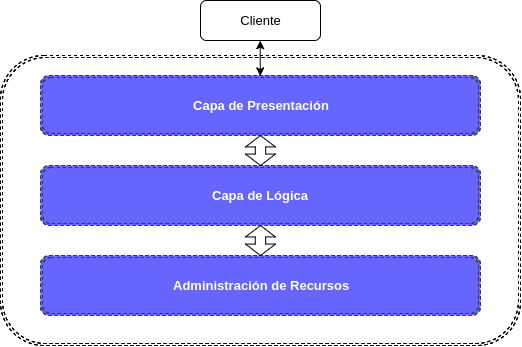
\includegraphics[scale=0.8]{DistArch}
  \end{center}
  \caption{Arquitectura de un Sistema Distribuido}
\end{figure}

\subsection{ Arquitecturas distribuidas modernas }
Como se mencionó en el punto anterior, los sistemas de información modernos utilizan estilos arquitectónicos distribuidos para mejorar el rendimiento, construcción y mantenimiento. A continuación se presentan las principales arquitecturas distribuidas: 

\subsubsection{ Cliente-Servidor }
Esta arquitectura distribuida reparte los requerimientos de procesamiento entre dos entidades, una que brinda servicios y recursos, llamada servidor y una que solicita esos servicios, llamada cliente.
Una de las principales ventajas de esta arquitectura no se refiere al rendimiento del sistemas sino a que permite una separación de responsabilidades y un esquema centralizado de las capas que lo conforman. Esta arquitectura permite a las organizaciones mantener un control sobre los equipos de trabajo que interfieren en la construcción de software, pues los equipos se dedican exclusivamente a modificar una parte del sistema. Si los equipos no mantienen un estándar ni expresan correctamente las especificaciones de la capa que desarrollan, el sistema puede tener problemas de integración.

\subsubsection{ N-Capas }
 Las arquitecturas a n-capas (también referenciadas como tiers, tercios o niveles) se presenta como una extensión al modelo clásico de 3 capas. En esta arquitectura se vinculan múltiples subsistemas creados debido a la complejidad que las capas pueden adquirir, por ejemplo, la capa de recursos tradicionalmente consiste en un sistema de base de datos, esta puede ser sustituida por un sistema de dos o tres capas donde se centralicen varias BD. Otra capa que se puede extender es la de presentación. Para distribuir eficientemente los procesos del sistema se puede implementar un servidor web encargado de generar las páginas html solicitadas por los clientes.
Conforme se van añadiendo más capas a los sistemas de información también se hace más complejo su desarrollo, mantenimiento y gestión.

\subsubsection{ SOA }
La arquitectura SOA (Service Ortented Architecture) es utilizada para crear sistemas distribuidos, permite una alineación directa de los procesos o lógica de negocio de las organizaciones con las funciones que ofrecen los sistemas desarrollados. Este tipo de sistemas permite una alta escalabilidad al  abstraer la lógica de negocios en Servicios. Los servicios son interfaces, por lo que no se describe la tecnología ni el funcionamiento interno de estos, sino que describen el comportamiento. Por lo regular  los servicios de una arquitectura SOA se implementan como WebServices, los cuales son un conjunto de tecnologías utilizadas para transferir datos entre aplicaciones a través de Internet, pueden utilizar distintos estándares, como XML, REST, etc.
Los servicios web en una arquitectura SOA permiten tener bien definida la manera en que se exponen y consumen los servicios, por lo que la integración de todas las capas del sistema se estandariza y facilita.

\subsection{ Transferencia de conocimiento en MBN }
En la empresa MBN actualmente la transferencia de conocimiento respecto a la arquitectura de las sistemas de información que desarrollan se lleva a cabo de manera genérica, pues se da un panorama amplio de cómo está conformada la arquitectura, pero no se cuenta con una guía institucional que cubra aspectos como: configurar el ambiente de desarrollo, comprobar que el ambiente de desarrollo se ejecute correctamente y desarrollar un proyecto integrador para familiarizarse con las tecnologías utilizadas.Según estudios internos la transferencia de conocimientos básicos sobre la arquitectura de aplicaciones de MBN requiere de 4 a 8 meses.

\section{ Justificación }
Para que un sistema de información SOA se pueda desarrollar sin inconvenientes, es necesario que todos los involucrados adopten la arquitectura y conozcan todos los componentes que la integran.
La propuesta de una arquitectura formal para los sistemas desarrollados en MBN optimizará el tiempo requerido para adoptarla, también facilitará una de las partes más importantes dentro de una empresa de  TI: la transferencia de conocimiento. 

\section{ Objetivos }
El objetico general de esta tesis es desarrollar una propuesta de arquitectura SOA para los sistemas de información desarrollados en MBN
Para alcanzar el objetivo general se plantean los siguientes objetivos específicos:
\begin{itemize}
\item Analizar y caracterizar las principales tecnologías utilizadas en los sistemas ya desarrollados por MBN.
\item Documentar la propuesta de Arquitectura 
\item Elaborar un documento formal que facilite la adopción de la arquitectura de MBN
\end{itemize}